\chapter{Evaluation}
\label{chap:evaluation}
%\noteinfo[inline]{Remember to describe that we could not get the network stack down on the FPGA}
\section{Setup}
In the initial stages of testing, the components had simulation processes between
block. This made it possible to implement different blocks of the system
independent of each other.\\
These tests were changing a lot because the initial design was not
reached.
When the modules were done, they were wired together and a simulator
was created to handle all input and output of the system.

\subsection{Graph file simulator}
\begin{figure*}%[!ht]
    \centering
    \begin{subfigure}[b]{0.16\textwidth}
        \centering
        \includegraphics[scale=0.45]{evaluation/dot_files/datain.eps}
        \caption{Data In}
        \label{fig:packet_graph_datain}
    \end{subfigure}%
    \begin{subfigure}[b]{0.16\textwidth}
        \centering
        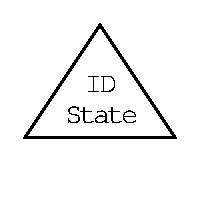
\includegraphics[scale=0.45]{evaluation/dot_files/send.eps}
        \caption{Send}
        \label{fig:packet_graph_send}
    \end{subfigure}%
    \begin{subfigure}[b]{0.16\textwidth}
        \centering
        \includegraphics[scale=0.45]{evaluation/dot_files/command.eps}
        \caption{Command \protect\footnotemark}
        \label{fig:packet_graph_command}
    \end{subfigure}%
    \begin{subfigure}[b]{0.16\textwidth}
        \centering
        \includegraphics[scale=0.45]{evaluation/dot_files/dataout.eps}
        \caption{Data Out}
        \label{fig:packet_graph_dataout}
    \end{subfigure}%
    \begin{subfigure}[b]{0.16\textwidth}
        \centering
        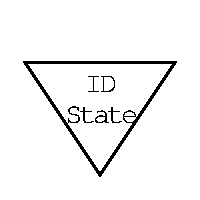
\includegraphics[scale=0.45]{evaluation/dot_files/receive.eps}
        \caption{Receive}
        \label{fig:packet_graph_receive}
    \end{subfigure}%
    \begin{subfigure}[b]{0.16\textwidth}
        \centering
        \includegraphics[scale=0.45]{evaluation/dot_files/wait.eps}
        \caption{Wait}
        \label{fig:packet_graph_wait}
    \end{subfigure}%
    \caption{The different node types in the simulation graph}
    \label{fig:packet_dot_files}
\end{figure*}%
The graph simulator is an abstract structure for easily composition and
illustrations of simulations in the system. The system can be boiled down
to inputs(sources) and output(sinks). The code is deterministic, since the same
combination of input and output signals would result in the exact same internal
state of the system. This means that a simulation of the system as a whole would
require knowing what to write/read at every source/sink, and doing it at the
right time. However, we do not need the timing on a clock to clock basis, since
the external network does not care when the system sends out a packet, only
if the packet is structured correctly. The user however may need information
regarding the latency of the system. The latency is based on the
specific system state, and is described in
\autoref{subsec:latency}.\\
With these assumptions it is possible to illustrate the timeline of the packets
with a graph, where a vertex does action on a clock to clock basis(etc. sending a
packet into the system.), and each edge describes what node to proceed to.
Each vertex have a state. When the \texttt{Done} state is reached
the next vertex is set to the \texttt{Ready} state, but only if
they are connected via an edge. If a vertex contains multiple ingoing edges, each
vertex with outgoing edges to that vertex needs to be \texttt{Done}.\\
{\renewcommand{\arraystretch}{1.3}
\begin{table}[htpb]
    \begin{center}
        \begin{tabular}{lcc}
            State & Color&Description\\ \hline \hline
            \texttt{Waiting}& \statecolorbox{graph_waiting} &
            \makecell{Vertex is not in use.}\\ \hline

            \texttt{Ready}& \statecolorbox{graph_isready} &
            \makecell{Vertex Is ready\\ for activation.}\\ \hline

            \texttt{Active}& \statecolorbox{graph_active} &
            \makecell{Vertex is active.\\ Simulator is\\ gathering data.}\\ \hline

            \texttt{Inactive}& \statecolorbox{graph_inactive} &
            \makecell{Vertex is inactive.\\Simulator is not\\ gathering data.}\\ \hline

            \texttt{Done}& \statecolorbox{graph_done} &
            \makecell{Vertex is done\\ and validated.}
        \end{tabular}
    \end{center}
    \caption{The different states of the nodes, and their respective colors
    used for illustration} \label{tab:graph_node_states}
  \end{table}
}\\
Each vertex have their own type, defining what input source or output sink to
use. The graph file simulator consists of multiple input sources and output sinks
as seen in \autoref{fig:packet_dot_files}.\\
There are three inputs giving data to the system:
Data in(\subref{fig:packet_graph_datain}),
Send(\subref{fig:packet_graph_send}) and
Command(\subref{fig:packet_graph_command}).
There are two sinks getting data from the system
Data out(\subref{fig:packet_graph_dataout}) and
Receive(\subref{fig:packet_graph_receive}).
The node type Wait(\subref{fig:packet_graph_wait}) is special, since
it does not use a input or a sink. It simply counts down each clock, until it's
counter reaches zero.\\
Since there only exist one of each input source and output sink (except Wait),
the simulator can only work on one vertex of each type at a time.
In graphs where there are multiple ready vertexes of same type, the vertex with
the lowest ID are focused on first. When a vertex is focused, it is set as
\texttt{Active}.\\
When the vertex is finished, it is set to \texttt{Done}.
An example of a graph can be seen in
\autoref{fig:graph_simulation_running_examples}.


\begin{figure*}[htpb]
    \centering
    \begin{subfigure}[b]{0.5\textwidth}
        \centering
        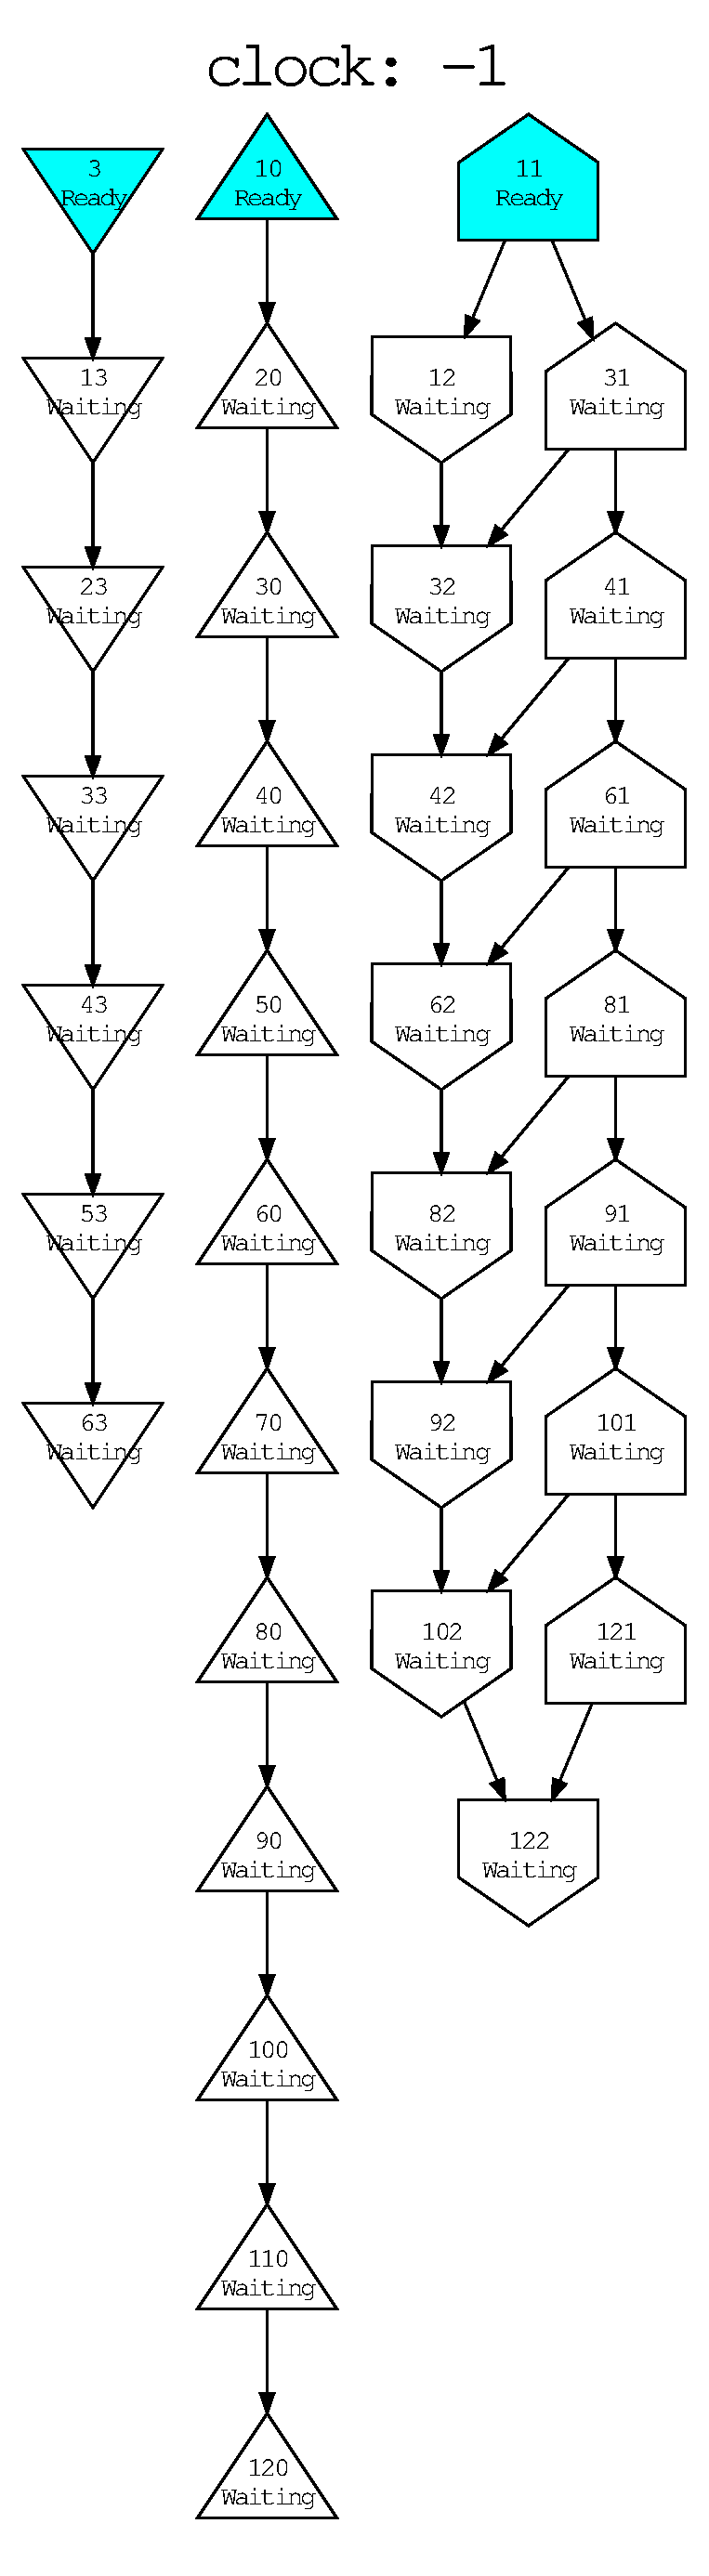
\includegraphics[scale=0.45]{evaluation/dot_files/example_graph_initial.eps}
        \caption{The initial state of a simulation}
        \label{fig:example_packet_graph_initial}
    \end{subfigure}%
    \begin{subfigure}[b]{0.50\textwidth}
        \centering
        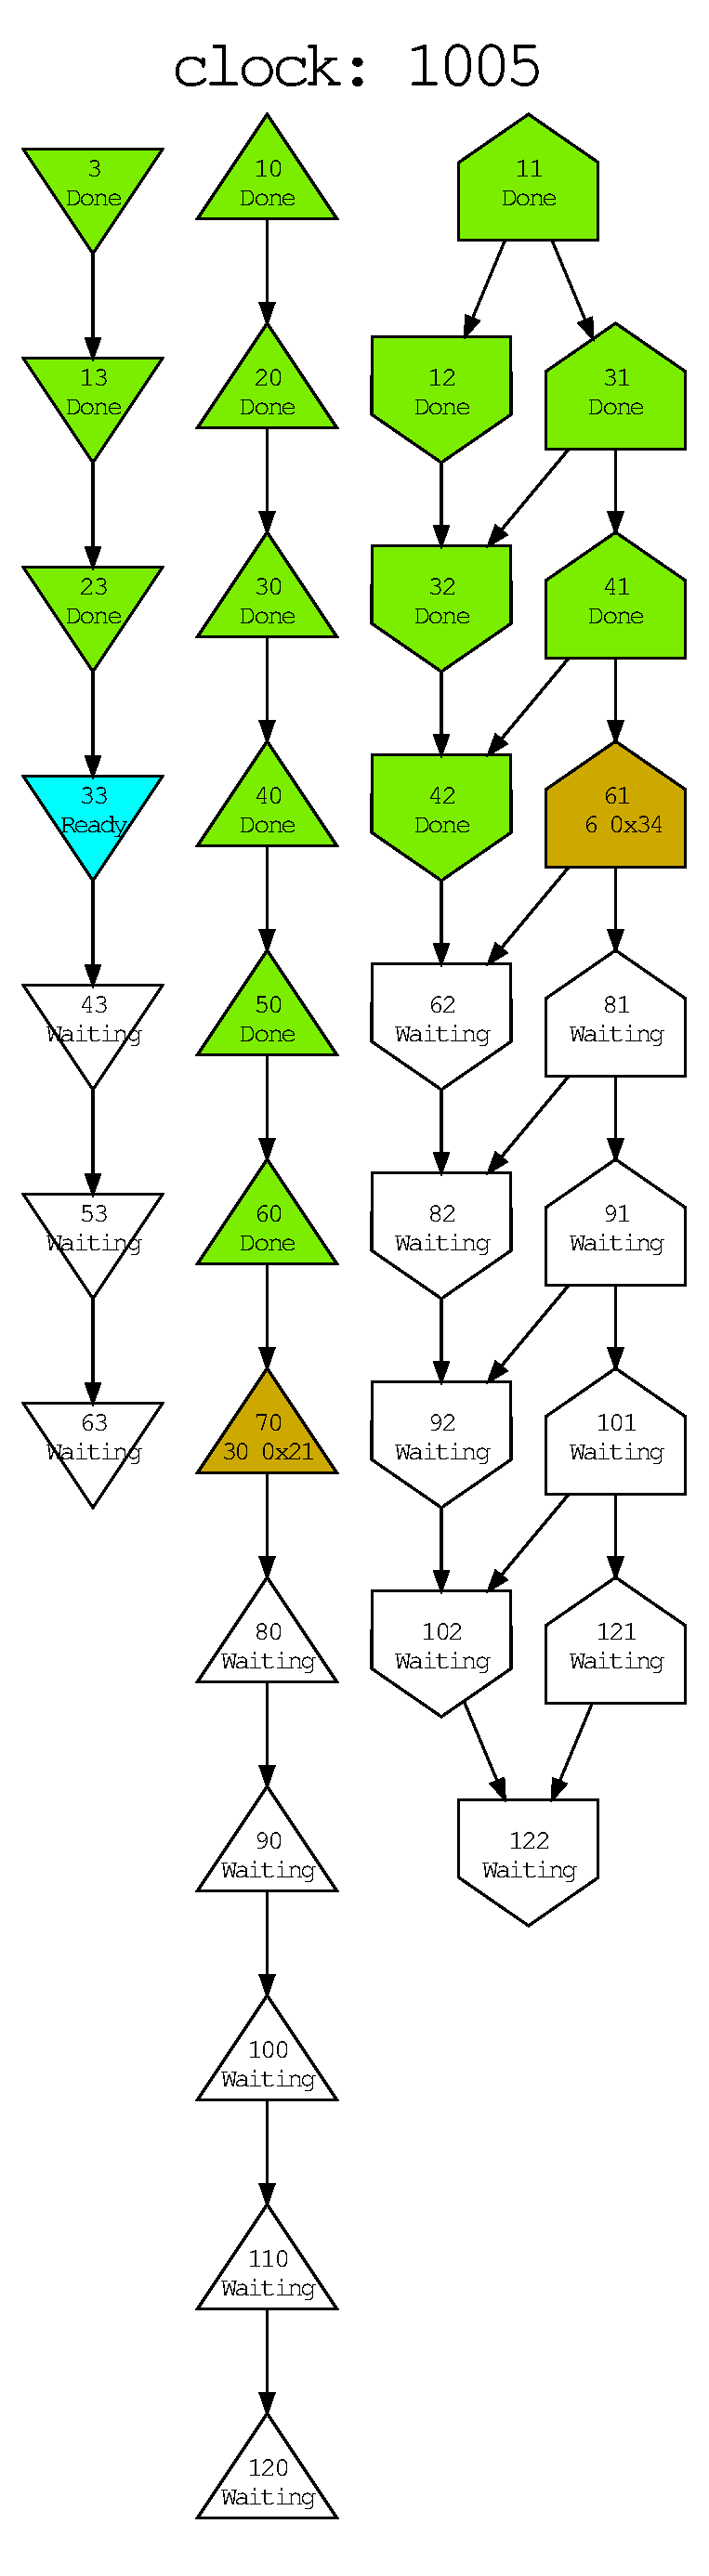
\includegraphics[scale=0.45]{evaluation/dot_files/example_graph_running.eps}
        \caption{The state after 1005 clocks}
        \label{fig:example_packet_graph_running}
 	\end{subfigure}%
    \caption{A Illustration of the graph states before running and 1005 clocks
    inside the simulation}
    \label{fig:graph_simulation_running_examples}
\end{figure*}

\subsection{VHDL code}
\notejan{should we add more to this?}
One of the biggest advantages of \gls{sme} is its easy testing, and its
compilation to VHDL code. By using the GHDL project
\cite{github_ghdl}\notemark{"By using the GHDL project, the generated VHDL code can be simulated to ensure that it is clock cycle accurate with the SME simulation" - eller noget i den dur}.
Unfortunately, our code does not compile into \gls{vhdl}.
\noteimprovement{Actually test with last revision of code}


\section{Test}
\footnotetext{This block is not implemented in the codebase}
% OBS, footnote text here from fig:packet_dot_files. needs to be on same page to work
To test the system we recorded a setup of packets containing both \gls{udp} and
\gls{tcp} packets, with focus on the \gls{udp} packets. There are three
\gls{udp} connections, and three \gls{tcp} connections. Two of the \gls{udp}
connections contain valid ports(6543,6789) and one contains an invalid port (3456).\\
Each of the valid udp connections where hardcoded into the test, so there where no
need for command blocks(\autoref{fig:packet_graph_command}).
In the illustration at \autoref{fig:graph_simulation_running_examples} the
same test is run, but with only $4*2$ good \gls{udp} packets, $4$ bad, and
no \gls{tcp} packets\\
When data is received from \texttt{Data In}, the same data is copied and
sent to \texttt{Data Out}. \\
In the example 6 packets have been sent into the system, and number 7(Id 70)
is \texttt{Active}. The active \texttt{Send} block is giving its 30'th byte
with a hex value of 0x21.\\
The real test had 17283 packets in total, where 1920 of those where udp packets.
Of the udp packets $2/3$ (1280) where the valid ports. The data sent
through \texttt{Internet In} totals 1832958 Bytes.\\
The test took around 1.83 million clocks to finish. This indicates that the system
did handle all incoming packets in real time without having to break the input,
even when sending limited amounts of data out.



\section{Verification}
\subsection{Latency}\label{subsec:latency}
There are several factors when calculating the latency of the system.
\begin{description}
    \item[$n_{\mathtt{D}}$]:\quad
    The number of bytes in the data part of the protocol. This excludes both
    headers from transport and internet.
    \item[$n_{\mathtt{I}}$]:\quad
    The internet header size.
    \item[$n_{\mathtt{T}}$]:\quad
    The transport header size.
    \item[$n$]:\quad
    The total packet size.
\end{description}
When a packet is propagating through the system, most
of the latency comes from the buffers. All processes that connects
to a buffer, does work, and submits to a buffer works on the data in real time.
When possible, processes will pass the data straight ahead. For example, the
\texttt{Transport} process will first pass the data from \texttt{Data Out} to
the \texttt{Segment Out}, and then send the header. The passing state happens
while reading from the buffer. This only adds two clock cycles of delay between
\texttt{Data Out} and \texttt{Segment out}.
In the following cases, we assume simple system where either only packets are
being sent, or packets are being received.

\subsubsection{From Recive to Data In}
When the system starts to receive the first byte of a packet, to the last byte read from
the user. This case uses \gls{ipv4} internet header, and \gls{udp} transport
header. This formular can also be used in other transport headers, such as \gls{tcp}.
To make it work with \gls{tcp}, one would need to calculate the constant $C$,
based on \gls{tcp} specific features such as how long are the sequence of
SYN/ACK \notemark{Carl var ogsaa forvirret over denne del. Jeg synes vi skal
slette TCP fra beregningen, for den er slet ikke implementeret.} takes.
\begin{equation*}
    2 + n + 2 + (n_{\mathtt{D}} + n_{\mathtt{T}}) + 2 + n_{\mathtt{D}}  + C
\end{equation*}
That simplifies down to
\begin{equation} \label{eq:receive_to_datain}
    C + 6 + n_{\mathtt{I}} + 2n_{\mathtt{T}} + 3n_{\mathtt{D}}
\end{equation}
\subsubsection{From Data out to Send}
Making the system send out data makes the formular a bit different. The outgoing
packets goes through an extra buffer.
\begin{equation*}
   2 + n_{\mathtt{D}} + 2 + (n_{\mathtt{D}} + n_{\mathtt{T}}) + 2 + n + 2 + n + C
\end{equation*}
That simplifies down to
\begin{equation} \label{eq:dataout_to_send}
    C + 8 + 2n_{\mathtt{I}} + 3n_{\mathtt{T}} + 4n_{\mathtt{D}}
\end{equation}

\subsubsection{Observations}\notemark{Noget andet, som i ikke har nævnt, at det i skriver er latency fra data kommer ind/ud til den er færdig. Jeres løsning er vel pipelinet, så efter start latency, så kan i vel blive ved med at feede netværket (hvad enten det er ind eller ud) ? }
It is clear when comparing \autoref{eq:dataout_to_send} and
\autoref{eq:receive_to_datain} that sending packets have a higher latency than
receiving packets. This is clearly because of the added buffer. It is not clear
from the latency formulars that receiving data "cuts" off data from the packet
at each buffer step. This makes it possible to receive data at a constant pace,
without filling the buffers. On the other hand sending out packets are
problematic. \\
Since each step adds additional information to the packet, the \texttt{Data Out}
buffer may fill faster than it can be emptied.


\subsection{Outgoing packet validation}

\begin{figure}[h]
\centering
\includegraphics[scale=0.45]{evaluation/hexdump.pdf}
	\caption{The hexadecimal representation of one of the outgoing packets
	generated by the system. Notice the red fields, indicating an error.}
\label{fig:packet_hexdump}
\end{figure}

The test has demonstrated that the packets themselves arrive at their
appropriate destinations intact. The test-suite tests all the supported
features, such as various protocols, port numbers, multiple connections through
sockets, etc.

To verify that the outgoing packets are formatted correctly, the output has
been captured and dumped into raw binary files. These can be interpreted by
numerous network utilities, such as the most well-known Wireshark.
These tools quickly detected malformations of the packets -- the
\texttt{protocol} field of the \gls{ipv4} header was not set, nor was the
destination address set. However, all offsets were calculated correctly, and
the packets had the exact proper lengths. Figure
\ref{fig:packet_hexdump} shows the raw binary dump of a packet, with the fields
marked.


\subsection{Internet Protocol Suite compliancy as per RFC 1122}
The networking stack was designed and implemented to comply with the networking
standards specified in RFC 1122. Although the number and size of the standards
required to be fully compliant with the Internet Protocol Suite is way over the
scope of this project, the list of requirements is a useful tool to get an
summary of the capabilities of the system.

Table \ref{tab:rfc_compliance} shows a subset of the required features.
Features and protocols unrelated to this project have been removed, and can be
assumed to not be supported. The full list can be seen in \cite[Section 3.5,
Page 72]{RFC1122}.
    \onecolumn
	\begin{longtable}{ | p{.30\textwidth} | p{.10\textwidth} | p{.025\textwidth} |  p{.025\textwidth} | p{.05\textwidth} | p{.40\textwidth} |}
\hline
	\textbf{Feature} & \textbf{RFC 1122 Section} &
		\rotatebox{270}{\textbf{must}} &
		\rotatebox{270}{\textbf{must not}} &
		\rotatebox{270}{\textbf{Compliance }} &
        \textbf{Comment} \\ \hline
\textbf{General} \\ \hline
Implement IP and ICMP                            &3.1     &x& & \cellcolor{yellow!25} & Partial; ICMP not supported \\ \hline
Handle remote multihoming in application layer   &3.1     &x& & \cellcolor{red!25 }& \\ \hline
Silently discard IP version != 4                 &3.2.1.1 &x& & \cellcolor{green!25 }& All versions except 4 are discarded\\ \hline
Verify IP checksum, silently discard bad datagrams &3.2.1.2 &x& & \cellcolor{yellow!25} & Discarding of bad datagram implemented but not enabled in current version\\ \hline

\textbf{Addressing} \\ \hline
  Subnet addressing (rfc-950)                    &3.2.1.3 &x& & \cellcolor{red!25 }\\ \hline
  Src address must be host's own IP address      &3.2.1.3 &x& & \cellcolor{green!25 } & Source address currently hardcoded\\ \hline
  Silently discard datagram with bad dest addr   &3.2.1.3 &x& & \cellcolor{red!25 }& No checks on addresses done\\ \hline
  Silently discard datagram with bad src addr    &3.2.1.3 &x& & \cellcolor{red!25 } & No checks on addresses done\\ \hline

\textbf{TOS} \\ \hline
Allow transport layer to set TOS              &3.2.1.6 &x& & \cellcolor{red!25 }& There is currently no communication between \texttt{Transport} and \texttt{Internet Out}\\ \hline

\textbf{TTL} \\ \hline
  Send packet with TTL of 0                      &3.2.1.7 & &x& \cellcolor{green!25 }& Hardcoded TTL is above 0\\ \hline
  Discard received packets with TTL $ < 2$          &3.2.1.7 & &x& \cellcolor{green!25 }& Ingoing TTL is ignored\\ \hline
  Allow transport layer to set TTL               &3.2.1.7 &x& & \cellcolor{red!25 }&\\ \hline
  Fixed TTL is configurable                      &3.2.1.7 &x& & \cellcolor{green!25}& TTL is configurable during compilation\\ \hline

\textbf{IP options} \\ \hline
  Allow transport layer to send IP options       &3.2.1.8 &x& & \cellcolor{red!25 }& There is currently no communication between \texttt{Transport} and \texttt{Internet Out}\\ \hline
  Pass all IP options received to higher layer       &3.2.1.8 &x& & \cellcolor{red!25 }& There is currently no communication between \texttt{Transport} and \texttt{Internet In}\\ \hline
  IP layer silently ignore unknown options       &3.2.1.8 &x& & \cellcolor{yellow!25}& All options are ignored\\ \hline
  Silently ignore stream identifer option        &3.2.1.8b&x& & \cellcolor{yellow!25 }& All options are ignored\\ \hline

\textbf{Source route option} \\ \hline
  Originate \& terminate source route options     &3.2.1.8c&x& & \cellcolor{red!25 }& Not implemented\\ \hline
  Datagram with completed sr passed up to tl     &3.2.1.8c&x& & \cellcolor{red!25 }& Not implemented\\ \hline
  Build correct (non-redundant) return route     &3.2.1.8c&x& & \cellcolor{red!25 }& Not implemented\\ \hline

\textbf{Reassembly and fragmentation} \\ \hline
  Able to reassemble incoming datagrams          &3.3.2   &x& & \cellcolor{green!25}& \texttt{Segment In} ensures that fragmented IP datagrams are reassembled before passing to transport layer\\ \hline
    -at least 576 byte datagrams                  &3.3.2   &x& & \cellcolor{green!25}\\ \hline
  Send icmp time exceeded on reassembly timeout  &3.3.2   &x& & \cellcolor{red!25 }& Not implemented\\ \hline

\textbf{Interface} \\ \hline
  Allow transport layer to use all IP mechanisms &3.4     &x& & \cellcolor{red!25 } & Transport cannot communicate with the IP layer  \\ \hline
  Pass interface ident up to transport layer     &3.4     &x& & \cellcolor{yellow!25 } & The identity of the interface is implicit from the \texttt{Segment In} bus \\ \hline
  Pass all IP options up to transport layer      &3.4     &x& & \cellcolor{red!25 } & IP options are not propagated from the IP layer\\ \hline
  Transport layer can send certain ICMP messages &3.4     &x& & \cellcolor{yellow!25 } & Theoretically; the transport layer can send any protocol out of the system\\ \hline
  Pass spec'd ICMP messages up to transport layer  &3.4     &x& & \cellcolor{red!25 }& Internet layer currently only handles IP datagrams \\ \hline
   -include IP header+8 octets or more from the original packet  &3.4     &x& & \cellcolor{red!25 } & \\ \hline
\hline
\caption{Compliance of a subset of the applicable requirements from RFC 1122}
\label{tab:rfc_compliance}
\end{longtable}
\twocolumn


